En esta sección se presentarán diversos artículos de investigación o tesis las cuales abordarán diversas técnicas y enfoques que se emplearon para afrontar problemas similares al de esta tesis.
% Asimismo, a continuación se presenta un cuadro resumen (véase Anexo \ref{A:table}) de lo que se presenta en esta sección.


%\subsection{Copper price estimation using bat algorithm \citep*{pr_dehghani2018copper}}

%\citeauthor{pr_dehghani2018copper} realizaron un artículo de investigación el cual fue publicado en la revista «Resources Policy» en el año 2018. Este fue titulado \citetitle{pr_dehghani2018copper} la cual traducida al español significa «Estimación del precio del cobre utilizando el algoritmo bat».

\subsection{Tesis relacionadas}
\subsection{Sales forecasting using long short term memory networks}

\subsubsection{Planteamiento del Problema y objetivo }
La tesis se enfoca en predecir las ventas de la empresa Annapolis Cider Company en Wolfville, Nova Scotia, con el objetivo de optimizar la asignación de recursos humanos. Se busca desarrollar un modelo de pronóstico que pueda predecir las ventas diarias y por hora con un margen de error del 10%. Se plantea que la precisión del 90% en las predicciones permitiría a la empresa gestionar sus recursos humanos de manera más eficiente.
Para abordar este desafío, se utilizan técnicas de aprendizaje automático, específicamente redes neuronales LSTM, que son conocidas por su eficacia en problemas de series temporales. Además de los datos históricos de ventas, el modelo también considera información como la fecha y hora, datos meteorológicos, indicadores de apertura/cierre y eventos especiales. Se comparan varios modelos de pronóstico, incluido un modelo de línea base de persistencia, un modelo Avg6Week y un modelo ARIMA, con el modelo LSTM para evaluar su rendimiento en la predicción de ventas minoristas.
Se reconoce que las ventas de cidra pueden presentar más variabilidad en comparación con las ventas de restaurantes debido a la naturaleza menos predecible de las ventas por hora. Además, se menciona que condiciones climáticas extremas, como tormentas y huracanes, pueden aumentar la dificultad de predecir con precisión las ventas


\subsubsection{Base de datos de los autores}
En la tesis se utilizan varios conjuntos de datos para el análisis y la predicción de ventas de la empresa Annapolis Cider Company. Estos conjuntos de datos incluyen:
Datos de ventas históricas almacenados en el sistema POS de la empresa para un período de hasta cuatro años.
Datos meteorológicos observados y pronosticados obtenidos del sitio web Dark Sky a través de un sitio web de recopilación de datos meteorológicos desarrollado llamado Weather Archive.
Datos de eventos especiales extraídos de varios calendarios en línea de la web, como Annapolis Valley Events, Office Holidays y Acadia Athletic.
Estos conjuntos de datos se utilizan para entrenar y evaluar los modelos de pronóstico, incluidos los modelos LSTM, ARIMA, persistencia y Avg6Week, con el objetivo de predecir las ventas diarias y por hora de la empresa


\subsubsection{Metodología empleada por los autores}
En la metodología siguen diversos pasos para el análisis y pronostico.
\begin{itemize}
	\item Data Collection: En la fase de Recopilación de Datos, se adquirieron datos de ventas históricas de la empresa Annapolis Cider Company almacenados en su sistema POS, datos meteorológicos observados y pronosticados de Dark Sky a través de Weather Archive, y datos de eventos especiales de fuentes en línea. Estos conjuntos de datos se utilizaron para el análisis y la predicción de ventas.
	\item Data Cleaning: El proceso de Limpieza de Datos involucró la detección y eliminación de valores irrelevantes, outliers, valores faltantes y duplicados en los conjuntos de datos de ventas y clima. Se realizó una conversión de tipos de datos y se calcularon las ventas por hora y por día a partir de los datos de transacciones originales.
	\item Descriptive Statistical Analysis: El Análisis Estadístico Descriptivo se centró en crear resúmenes y medidas de los datos de ventas antes de desarrollar los modelos predictivos. Se utilizaron gráficos para analizar las ventas en diferentes escalas de tiempo y se identificaron patrones estacionales y tendencias en los datos.
	\item Data Preparation: En la etapa de Preparación de Datos, se realizaron acciones como la estacionalización de datos, la selección de características relevantes, la creación de un indicador de eventos especiales, la normalización de datos y la división de datos en conjuntos de entrenamiento, validación y prueba. Además, se prepararon los datos de entrada para los modelos de pronóstico.\\
	
	A continuación, se presenta un resumen detallado de los métodos de modelado de predicción utilizados:
	
	\item Persistence Model:
	En el modelo de persistencia, la predicción de ventas para el próximo día (o próxima hora) es exactamente igual a las ventas del día (o hora) actual. Este enfoque es un modelo de referencia estándar para series temporales y solo puede hacer predicciones a corto plazo.
	\item Avg6Week Model:
	En este enfoque común, se calcula el promedio de las ventas en el mismo día de la semana durante las últimas 6 semanas para predecir las ventas del próximo día. Este modelo proporciona predicciones para cualquier día de la semana en la próxima semana.
	
	\item ARIMA Model:
	Se desarrolló un modelo ARIMA (Autoregressive Integrated Moving Average) que utiliza las ventas de los últimos 7 días para predecir las ventas del día siguiente. Este enfoque se basa en la identificación de patrones en los datos de series temporales.
	
	\item LSTM Neural Networks:
	Se implementó una red neuronal LSTM (Long Short-Term Memory) recurrente que utiliza datos de ventas, variables de fecha y hora, condiciones meteorológicas observadas, indicadores de apertura/cierre e indicadores de eventos especiales de los últimos 7 días, junto con el pronóstico del clima para el día siguiente. Este modelo se desplaza en el tiempo para hacer predicciones a dos días en el futuro.
	
	
\end{itemize}

\subsubsection{Resultados obtenidos}

\begin{itemize}
	\item Daily Sales Prediction Results:
	El modelo LSTM para predicción diaria de ventas mostró el menor error absoluto medio (MAE) en el conjunto de prueba, con un valor de \$597.93 y un error porcentual absoluto medio (MAPE) del 19.7\%. Esto representó una reducción del 22.6\% en el error de prueba en comparación con el modelo de persistencia diaria.
	
	\item Hourly Sales Prediction Results:
	Para la predicción por hora de las ventas, el modelo LSTM logró el menor MAE en el conjunto de prueba, con un valor de \$51.59 y un MAPE del 40.8\%. Esto representó una disminución del 17.2\% en el error de prueba en comparación con el modelo de persistencia por hora.
	
	\item Comparative Analysis:
	Se observó que el modelo LSTM superó significativamente a los modelos de persistencia, Avg6Week y ARIMA en términos de precisión de predicción tanto para las ventas diarias como por hora. La capacidad de la red neuronal LSTM para capturar patrones complejos en los datos de series temporales y su capacidad para aprender de secuencias largas contribuyeron a su rendimiento superior.
	
	\item Impact of LSTM Features:
	La inclusión de variables como datos de ventas históricas, fecha y hora, condiciones meteorológicas observadas, indicadores de apertura/cierre y eventos especiales en el modelo LSTM demostró ser crucial para mejorar la precisión de las predicciones de ventas. Estos factores externos y temporales permitieron al modelo LSTM capturar mejor la variabilidad en los datos de ventas.
	
\end{itemize}

%%%%%%%%%%%%%%%%%%%%%12

%\subsection{Estudio sobre Pronósticos de Ventas utilizando Series Temporales del Producto Nutrileche de la Empresa "Decar" S.A}
%
%Rodríguez, T (2018), en su estudio, ubicada en la ciudad de Machala. \textbf{Objetivo:} Conocer el pronóstico de ventas del producto en la empresa mediante el uso de series temporales. \textbf{Metodología}: El enfoque utilizado en el estudio fue de campo, empleando un modelo estadístico y técnicas cuantitativas. \textbf{Resultados:} Al aplicar el método del promedio móvil simple, se proyectó que las ventas para noviembre de 2017 alcanzarían los \$ 59352,99, con una desviación estándar de \$2834,61. Se tomaron en cuenta datos históricos desde octubre de 2016 hasta octubre de 2017. \textbf{Conclusiones:} Se llevaron a cabo tres métodos de pronóstico de ventas utilizando series temporales: promedio móvil simple, promedio móvil ponderado y suavización exponencial simple. Mediante diversas proyecciones, se obtuvieron datos significativos para análisis y toma de decisiones precisa.

\subsection{Investigación sobre Implementación de un Sistema de Pronóstico de Ventas utilizando Redes Neuronales Artificiales para la Empresa Cerámicos Lambayeque SAC}


\subsubsection{Planteamiento del Problema y objetivo}
La investigación presenta la implementación de un sistema basado en redes neuronales artificiales (RNA) para pronosticar las ventas en la empresa ``Cerámicos Lambayeque SAC''. Para esto, se emplean datos históricos de ventas diarias y mensuales correspondientes a los años 2016 y 2017. Estos datos, obtenidos de los sistemas transaccionales de la empresa, a menudo se encuentran en desorden, incompletos o manipulados. Sin embargo, las RNA son capaces de filtrar el ruido y manejar estos datos de manera efectiva.\\

Los datos de ventas se almacenan en un arreglo bidimensional estático de 200 filas por 5 columnas, donde las ventas de 2016 se guardan en las posiciones de 0 a 71, las de 2017 en las posiciones de 72 a 143, y las ventas pronosticadas para 2018 se almacenan desde la posición 144 hasta la 199. Cada venta diaria se normaliza dividiéndola entre 1000.\\

Durante el entrenamiento de la RNA, se visualizan las ventas pronosticadas y se ajustan los pesos sinápticos iniciales. La estructura de la red neuronal consiste en cuatro neuronas de entrada, doce neuronas ocultas y una neurona de salida. Los atributos de la red se definen y se asignan valores a través de matrices para los pesos sinápticos. El entrenamiento de la RNA incluye la asignación de datos de ventas y un número determinado de iteraciones, así como la definición del ratio de aprendizaje. Durante cada iteración, se obtienen y visualizan los errores de predicción. El software permite al usuario comparar las ventas históricas y pronosticar las ventas diarias desde enero hasta julio de 2018.

\subsubsection{Base de datos de los autores}

Las ventas realizadas por la empresa durante los años 2016 y 2017. Esta información, que se encuentra en la base de datos de la empresa, será utilizada para realizar el pronóstico.Las ventas diarias y mensuales de los años 2016 y 2017 se almacenan en un arreglo bidimensional estático de 200 filas por 5 columnas. Las ventas de 2016 se ubican desde el ítem 0 hasta el ítem 71, mientras que las ventas de 2017 se colocan desde la posición 72 hasta la posición 143. Finalmente, las posiciones desde la 144 hasta la 199 se reservan para las ventas diarias y mensuales pronosticadas para el año 2018.

\subsubsection{Metodología empleada por los autores}
\begin{enumerate}
	\item Definición del Almacén de Ventas:
	Se estableció una estructura bidimensional para registrar las ventas diarias mensuales, organizadas en filas, con el fin de utilizarlas en el entrenamiento y predicción mediante la red neuronal.
	\item Creación de la Solución y Proyectos:
	Se empleó Microsoft Visual C\# 2013 para desarrollar la aplicación, configurando una solución inicial en blanco y proyectos específicos para la red neuronal y la aplicación de consola.
	\item Codificación del Sistema:
	Se detallaron los pasos necesarios para la programación del sistema de pronóstico de ventas, abarcando la definición de pesos y la visualización de datos de ventas durante el entrenamiento de la red neuronal.	 
	
	\item Entrenamiento de la Red Neuronal:
	Se realizó el entrenamiento de la red neuronal, estableciendo parámetros como el número máximo de épocas y creando arreglos para manejar los gradientes de salida e entrada, así como las señales de los nodos ocultos y de salida.
	
	\item Barajado de Datos:
	Se implementó un proceso para mezclar aleatoriamente los datos de ventas, visitando cada dato en un orden aleatorio para optimizar el entrenamiento de la red neuronal.
	
	\item Fijar Pesos:
	En esta etapa, se asignan los pesos previamente generados para la red neuronal, asegurando que los valores correctos se apliquen a los nodos de la red.
	
	\item Implementación de la Red:
	Se desarrolló una clase específica para la red neuronal, que incluye todas las funciones y métodos necesarios para predecir las ventas diarias mensuales.
	
	\item Definición de Atributos de la Clase:
	Se establecieron las variables que representan el número de nodos de entrada, nodos ocultos y nodos de salida de la red, además de matrices para almacenar las entradas y los pesos sinápticos.
	
	\item Inicialización de Pesos:
	Se generaron los pesos iniciales necesarios para el funcionamiento de la red neuronal, que se utilizan durante el entrenamiento y la predicción de ventas.
	
	\item Cálculo de Salidas Deseadas:
	Se llevaron a cabo cálculos específicos para determinar las salidas deseadas de la red neuronal, mejorando así la precisión de las predicciones de ventas.
\end{enumerate}

\subsubsection{Resultados obtenidos}


\begin{table}[H]
	\caption{Resultados de Ventas pronosticadas}
	\centering
	\begin{tabular}{C{2.5cm} C{3cm} C{3cm} C{3cm} }
		\hline 
		\textbf{Mes} & \textbf{Venta diaria S/.} & \textbf{Venta pronosticada con la red S/.} & \textbf{Grado de confiabilidad \%} \\
		\hline
		Enero & 670675 & 668705 & 99,71 \\
		\hline
		Febrero & 678351 & 645902 & 95,22\\
		\hline
		Marzo & 708787 & 663617 & 93,63\\
		\hline
		Abril & 701295 & 659217 & 94,00\\
		\hline
		Mayo & 701760 & 646789 & 92,17\\
		\hline
		Junio & 692871 & 650631 & 93,90\\
		\hline
		Julio & 704171 & 650239 & 92,34\\
		\hline
	\end{tabular}
	\newline
	 \newline \textit{Fuente: Benites Sernaqué, J. M. (2021). Implementación de un sistema de pronóstico de ventas utilizando redes neuronales artificiales para la empresa Cerámicos Lambayeque SAC.}
	\label{tab:reftesis2}
\end{table}

%\subsubsection{Planteamiento del Problema y objetivo}
%\subsubsection{Base de datos de los autores}
%\subsubsection{Metodología empleada por los autores}
%\subsubsection{Resultados obtenidos}


\subsection{Aplicativo Web de Series Temporales para el Pronóstico de Ventas en la Empresa SERMIMIN}

\subsubsection{Planteamiento del Problema y objetivo}
La tesis trata sobre la imprecisión en los pronósticos de ventas en varias empresas, incluida SERMIMIN, una consultora registrada en OSINERGMIN y OEFA. De acuerdo con varios estudios, muchos ejecutivos no valoran lo suficiente la importancia de predecir ventas, considerándolo impreciso y poco fiable para nuevos productos. No obstante, un pronóstico preciso es fundamental, ya que influye en la planificación de producción, compras, inventarios y ventas.\\

El uso insuficiente de herramientas de pronóstico, especialmente de software especializado, es un problema recurrente. Las empresas que carecen de software adecuado para predecir ventas experimentan deficiencias importantes. La inteligencia artificial (IA) y el aprendizaje automático proporcionan soluciones avanzadas para mejorar la precisión de los pronósticos. La IA permite a las computadoras imitar el pensamiento humano, comprender el lenguaje natural y realizar tareas complejas de manera eficiente. La implementación de modelos matemáticos y algoritmos de IA puede disminuir significativamente los errores de pronóstico.\\

En el caso de SERMIMIN, la empresa realiza sus pronósticos de manera empírica, lo que ha provocado errores y costos adicionales. La ausencia de un sistema de información adecuado para registrar y evaluar sus parámetros de servicio agrava estos problemas. Se desarrolla un aplicativo web utilizando redes neuronales para mejorar la precisión del pronóstico de ventas en SERMIMIN.

\subsubsection{Metodología empleada por los autores}
En esta investigación sobre el pronóstico de ventas, se registrarán las ventas realizadas por la empresa Sermimin, ingresando estos datos en el sistema para entrenar redes neuronales con información histórica de ventas. Posteriormente, se realiza el pronóstico según los servicios de la empresa. El sistema pasará por una fase de entrenamiento para identificar un modelo de pronóstico óptimo, utilizando indicadores de precisión para generar información confiable en los pronósticos de ventas de la empresa. En cuanto al método de análisis de datos en esta investigación utilizó un enfoque cuantitativo con un diseño pre-experimental. Además, se emplearon métodos estadísticos para validar o refutar las hipótesis planteadas en capítulos anteriores.

\subsubsection{Resultados obtenidos}
Como resultados se concluye que hubo una mejora significativa en el indicador de desviación media absoluta, que pasó de un valor de 625.83 antes de la incorporación del aplicativo de redes neuronales a 104.58 después de su implementación, reduciéndose en 521.83 puntos.
Además, se concluye que el indicador de error porcentual medio absoluto también mejoró considerablemente, pasando de un valor de 1568.0 antes de la implementación del sistema de redes neuronales a 2.9167 después, representando una mejora de 1348 puntos.
Como resultado final, el aplicativo web basado en redes neuronales mejora notablemente ambos indicadores, tanto la desviación media absoluta como el error porcentual medio absoluto, demostrando su efectividad en el pronóstico de ventas para la empresa Sermimin.	



\subsection{Análisis de Pronóstico de Demanda para la Gestión del Inventario en el Sector Salud}

\subsubsection{Planteamiento del Problema y objetivo}
En esta investigación optaron por diseñar preliminarmente un aplicativo web destinado a realizar pronósticos de la demanda futura de todos sus productos, utilizando conceptos de Machine Learning. Este enfoque permitiría prever con mayor precisión la demanda futura y serviría como soporte tecnológico para agilizar la toma de decisiones.

Como primer paso, la plataforma web se conectaría con la base de datos proporcionada por Amazon Web Services (AWS), donde se registraría toda la información de los usuarios y los algoritmos, incluidos los resultados de los pronósticos de demanda. Los algoritmos se implementarían utilizando el lenguaje de programación Python, conocido por su uso amplio y versatilidad en diversas industrias debido a su licencia de código abierto. Además, se emplearía Anaconda, una distribución de Python especializada en aplicaciones de ciencia de datos y Machine Learning, capaz de manejar grandes volúmenes de datos.

Para el desarrollo del modelo, se implementarían varios tipos de algoritmos y se seleccionaría el que ofreciera mayor precisión y aplicabilidad en el sector de la empresa. Los resultados se visualizarían mediante el servicio de Power BI, presentando diversos gráficos y tablas, como el plan de compras a futuro, accesibles desde una PC en cualquier momento.
%\subsubsection{Base de datos de los autores}

\subsubsection{Metodología empleada por los autores}

\begin{itemize}
	\item Etapa 01: \textbf{Empatizar. } 
	Se centró en comprender el comportamiento del usuario en la gestión de sus inventarios. Se llevaron a cabo diversas encuestas virtuales utilizando Google Forms, dirigidas a importadores y vendedores de materiales del sector salud. Estas encuestas recogieron opiniones sobre la gestión de inventarios, las herramientas utilizadas y la planificación de compras futuras. En total, se realizaron 60 encuestas, de las cuales el 36.6\% de los encuestados reportó contar con un sistema digital de inventarios en sus empresas.
	\item Etapa 02: \textbf{Definir. }
	En esta segunda fase, se identificaron las necesidades del cliente mediante encuestas y entrevistas, seleccionando los principales insights y necesidades clave que agregarían valor al proyecto. Descubrieron que el costo mensual o anual de las soluciones de gestión de inventarios era una preocupación importante para los usuarios, ya que a menudo resultaban inviables. Además, los usuarios preferían herramientas con un número reducido de módulos, ya que una complejidad excesiva podría desanimarlos a seguir utilizándolas debido al tiempo requerido para la capacitación.
	\item Etapa 03: \textbf{Prototipar. }
	Después de identificar y definir las necesidades de los usuarios, se diseñaron el storyboard y el prototipo, incluyendo capturas de la aplicación web. Estas actividades ayudaron a materializar las ideas seleccionadas mediante sesiones de brainstorming con los usuarios.
	\item Etapa 04: \textbf{Esquema del Prototipo Inicial. }
	La arquitectura del prototipo consistió en un aplicativo web que permitía a los usuarios acceder y conectarse al servicio web en la nube a través de Amazon Web Services (AWS) mediante un servicio API. Esto incluía bases de datos de usuarios, algoritmos y resultados. Para la validación de los clientes, se utilizó un servicio web llamado "Validar", donde los usuarios ingresaban su ID y contraseña para acceder al sistema. Una vez autenticados, los usuarios ingresaban datos iniciales a la base de datos de algoritmos a través del servicio web "Pronóstico" para encontrar el algoritmo más adecuado según los datos históricos proporcionados. Los algoritmos fueron desarrollados en Python, y los resultados se almacenaban en la base de datos de resultados, sirviendo de base para cálculos de pronósticos y mostrando diversos dashboards mediante Power BI.
	\item Etapa 05: \textbf{Evaluar. }
	Las evaluaciones del prototipo realizadas por los usuarios finales permitieron mejorar constantemente su diseño basado en sus observaciones y sugerencias. Se desarrollaron varias versiones del prototipo, destacando su simplicidad, la disposición de tablas y gráficos, y la importancia de los datos de entrada y salida para un pronóstico adecuado de la demanda futura. Estas mejoras aseguraron que la interacción con la plataforma web fuera ágil y fácil de manejar.
	
\end{itemize}


\subsubsection{Resultados obtenidos}
La solución se orienta específicamente hacia pequeñas y medianas empresas dedicadas a la importación y venta de productos de salud, así como a cadenas de farmacias y clínicas en las zonas 6, 7 y 8 de Lima Metropolitana, atendiendo a los Niveles Socioeconómicos (NSE) A, B, y C. La propuesta implica la instauración de una plataforma web que utiliza la infraestructura Cloud de almacenamiento de datos y la página web de Amazon Web Services (AWS), junto con un motor generador de información en tiempo real basado en Python, un modelo de aprendizaje supervisado y diversos paneles de control en Power BI para proyectar la demanda futura. El proyecto fue desarrollado en 63 días con una inversión de S/ 65,700 soles. Conclusión: La herramienta ha permitido a los usuarios realizar pronósticos precisos de la demanda futura, lo que ha llevado a una optimización de los niveles de inventario y una reducción de los costos operativos en un 30\%. Esto ha resultado en un aumento del 94\% en las utilidades y en la mejora del nivel de servicio.

%%%%%%%%%%%%%%%%%%%%%%%%

\subsection{Artículos relacionados}

\subsection{Time‑series analysis with smoothed Convolutional Neural Network}

\subsubsection{Planteamiento del Problema y objetivo }
La introducción del documento `Time-series analysis with Smoothed Convolutional Neural Network (SCNN)' comienza destacando la importancia del análisis de series temporales en diversas áreas, como las finanzas, la meteorología y la medicina, donde la capacidad de predecir y comprender patrones en datos temporales es fundamental para la toma de decisiones efectivas. Se menciona que las técnicas tradicionales de suavizado de datos pueden mejorar la calidad de las series temporales al eliminar valores atípicos y ruido.
Se introduce el concepto de Redes Neuronales Convolucionales (CNN), que son ampliamente utilizadas en el procesamiento de imágenes debido a su eficiencia en la extracción de características. El documento destaca que las CNN pueden ser aplicadas a problemas de series temporales al tratar los datos de entrada como arreglos unidimensionales, lo que las hace adecuadas para el análisis de datos temporales.
La motivación principal del estudio es explorar cómo la combinación de técnicas de suavizado de datos con CNN puede mejorar la precisión en la predicción de series temporales. Se plantea la hipótesis de que, al optimizar el factor de suavizado en CNN, se puede lograr un rendimiento superior en la predicción de series temporales en comparación con otros métodos tradicionales.\\


\begin{table}[H]
	\caption{Tipos de suavizado de datos (data smoothing)}
	\centering
	\begin{tabular}{L{4cm}|L{5cm}|L{5cm}}
		\hline 
		\textbf{Método} & \textbf{Ventajas} & \textbf{Desventajas}\\
		\hline
		Suavizado exponencial/Suavizado simple exponencial & Facilidad de cálculo, Flexibilidad, Buen rendimiento. & No es capaz de gestionar bien las tendencias.  \\
		\hline
		Media móvil & Uso adecuado cuando hay ligera o nula variación estacional. & Puede no reflejar con exactitud las tendencias más recientes.\\
		\hline
		Recorrido aleatorio & Fácil de usar, Puede manejar flujos complicados. & No conserva con precisión la posición media de la vorticidad en el espacio libre, Soluciones ruidosas debido a errores estadísticos.\\
		\hline
	\end{tabular}
	\newline
	\newline \textit{Fuente: Wibawa, A. P.(2022). Time-series analysis with smoothed Convolutional Neural Network. Journal of big Data, 9(1), 44.}
	\label{tab:metodos}
\end{table}


\subsubsection{Base de datos de los autores}
Se presentan 4 conjuntos de datos diferentes, cada uno con características específicas:\\
\begin{enumerate}
	\item Dataset 1: Se trata de una serie temporal de un año de visitantes diarios a un sitio web de la Universidad Negri Malang. Este conjunto de datos es multivariado y consta de 365 instancias con 4 atributos diferentes, como sesiones, visitas a páginas, visitantes y nuevos visitantes. 
	\item Dataset 2: Este conjunto de datos también es multivariado y consiste en datos diarios de visitantes a un sitio web, pero con diferentes atributos en comparación con el Dataset 1. Incluye información sobre cargas de página, visitas únicas, visitas por primera vez y visitas recurrentes.
	\item Dataset 3: Se refiere a datos relacionados con el intercambio de divisas y la información de ventas. Es un conjunto de datos multivariado con 2 atributos y no presenta datos faltantes.
	\item Dataset 4: Este conjunto de datos representa el consumo de energía eléctrica en 32 ciudades de la India. Es un conjunto multivariado con un atributo seleccionado para el estudio, que es la demanda de energía en Delhi.
	
	Además, se menciona que se utilizan dos escenarios diferentes para evaluar el rendimiento del modelo en función de la composición de los datos de entrenamiento y prueba. En el primer escenario dividen en 70\% y 30\% en el entrenamiento y prueba respectivamente, en el segundo escenario dividen 80 \% y 20\%.
\end{enumerate}


\subsubsection{Metodología empleada por los autores}
\begin{enumerate}
	\item Evaluación del método propuesto: Se inicia con la evaluación del método propuesto, que combina el suavizado exponencial con CNN (S-CNN). Se comparan los resultados obtenidos con S-CNN con los de otros métodos de pronóstico, como Multilayer Perceptron (MLP) y Long Short-Term Memory (LSTM). Se destaca que S-CNN supera a MLP y LSTM en términos de error cuadrático medio (MSE), con el mejor MSE logrado utilizando 76 capas ocultas.
	\item Comparación de desempeño: Se presentan los resultados de pruebas de significancia utilizando el test t pareado basado en el número de capas ocultas de Lucas. Se comparan métricas como MSE, MAPE y tiempo de entrenamiento entre CNN y S-CNN. Se observa que S-CNN es más preciso que CNN en todos los escenarios y que el tiempo de procesamiento es menor con S-CNN.
	\item Optimización del factor de suavizado: Se discute la importancia de encontrar el factor de suavizado óptimo ($\alpha$) en el método propuesto. Se comparan diferentes valores de $\alpha$ y se concluye que el $\alpha$ óptimo produce los mejores resultados en términos de MSE y MAPE.
	\item Impacto de las capas ocultas de Lucas: Se analiza el impacto de utilizar números de Lucas como capas ocultas en la CNN. Se muestra que las capas ocultas de Lucas tienen un efecto significativo en la precisión del modelo y en el tiempo de entrenamiento, mejorando el rendimiento del algoritmo de pronóstico.
\end{enumerate}

%%%%Ecuacion
%\begin{equation}  
%\label{eq:RMSE}
%RMSE = \sqrt{\frac{\sum_{i=1}^{N}{\Big(O_i -T_i\Big)^2}}{N}}
%\end{equation}

\begin{figure}[H]
	\begin{center}
		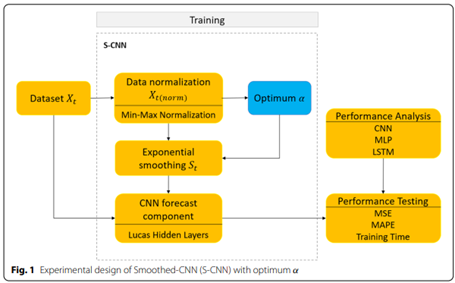
\includegraphics[width=0.7\textwidth]{2/figures/ant1_time-series.png}
		\caption{Metodologia antecedente}
		\textit{Fuente: Wibawa, A. P.(2022). Time-series analysis with smoothed Convolutional Neural Network. Journal of big Data, 9(1), 44.}
		\label{fig9}
	\end{center}	
\end{figure}

\subsubsection{Resultados obtenidos}
Se resalta que los resultados obtenidos en el estudio sugieren que la implementación de S-CNN con capas ocultas de Lucas puede elevar el rendimiento del algoritmo de pronóstico en el análisis de series temporales, reduciendo el error cuadrático medio (MSE) y mejorando la precisión de las predicciones.

\begin{figure}[H]
	\begin{center}
		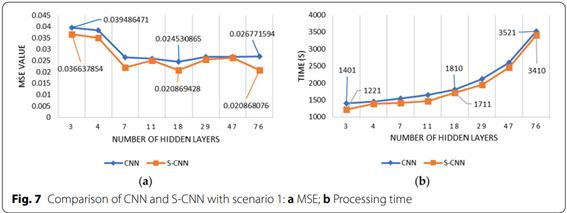
\includegraphics[width=0.7\textwidth]{2/figures/resul_ant1.png}
		\caption{Resultado antecedente}
		\textit{Fuente: Wibawa, A. P.(2022). Time-series analysis with smoothed Convolutional Neural Network. Journal of big Data, 9(1), 44.}
		\label{fig9}
	\end{center}	
\end{figure}

\begin{figure}[H]
	\begin{center}
		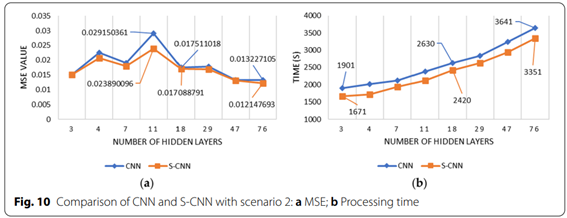
\includegraphics[width=0.7\textwidth]{2/figures/resul_ant11.png}
		\caption{Resultado antecedente}
		\textit{Fuente: Wibawa, A. P.(2022). Time-series analysis with smoothed Convolutional Neural Network. Journal of big Data, 9(1), 44.}
		\label{fig9}
	\end{center}	
\end{figure}



%%%%%%%%%%%%%%%%%%%2 

\subsection{Approaching sales forecasting using recurrent neural networks and transformers}

\subsubsection{Planteamiento del Problema y objetivo }
Se destaca el crecimiento del comercio electrónico y la importancia de mejorar los sistemas de cadena de suministro para satisfacer la creciente demanda en la industria minorista en línea. Se menciona que la precisión en la predicción de la demanda del cliente es fundamental para optimizar aspectos como la ubicación de inventarios, la expansión de la red y la planificación de entrada y salida. 
El artículo destaca la importancia de un pronóstico preciso y rápido de la demanda en la cadena de suministro para mejorar la ejecución de los procesos descendentes correspondientes, como la planificación de entrada y salida, la ubicación de inventarios y la planificación de la red. Los autores presentan tres alternativas basadas en técnicas de aprendizaje profundo para predecir las ventas de clientes a nivel de día, tienda y producto. Con esto propone el uso de técnicas de aprendizaje profundo, como redes neuronales recurrentes y transformers, para abordar el problema de pronóstico de la demanda de manera generalizada, permitiendo predecir las ventas para diferentes productos, ubicaciones y momentos con un solo modelo. Esto contrasta con otros enfoques, como los modelos de la familia ARIMA, que solo pueden manejar una serie temporal de producto-ubicación a la vez.


\subsubsection{Base de datos de los autores}
El conjunto de datos utilizado en este estudio es el conjunto de datos de ventas de supermercados de Corporación Favorita. Este conjunto de datos fue publicado como parte de una competencia de Kaggle y contiene registros de ventas diarias para 4400 artículos únicos en 54 tiendas ecuatorianas diferentes. Los datos abarcan desde el 1 de enero de 2013 hasta el 15 de agosto de 2017. Además de la información de ventas diarias, se proporcionan datos adicionales que incluyen detalles sobre la cantidad de ventas, las ubicaciones de las tiendas, la fecha, familia del artículo, precio del aceite y días festivos.

\subsubsection{Metodología empleada por los autores}
Se llevó a cabo una metodología experimental detallada que incluye los siguientes pasos:
Selección del conjunto de datos: Se utilizó el conjunto de datos proporcionado por la Corporación Favorita, que consta de una gran cantidad de muestras (alrededor de 400 Millones) que permiten el uso de modelos de aprendizaje profundo.
Diseño de arquitecturas: Se diseñaron dos arquitecturas neuronales diferentes para abordar el problema de pronóstico de ventas: un modelo seq2seq y un modelo transformer. Estas arquitecturas fueron adaptadas y modificadas para ajustarse específicamente al problema de pronóstico de ventas en el contexto de la Corporación Favorita.
Implementación de la arquitectura seq2seq: La arquitectura Seq2seq (sequence-to-sequence) es un modelo diseñado para mapear una secuencia de entrada a una secuencia de salida, sin restricciones en las longitudes de ambas secuencias. En el contexto del pronóstico de ventas, el modelo Seq2seq se utiliza para predecir las ventas diarias de productos en tiendas específicas. La arquitectura Seq2seq consta de dos componentes principales: el codificador y el decodificador. El codificador procesa la secuencia de entrada, que en este caso incluiría datos históricos de ventas y otras características relevantes, y condensa esta información en un vector de contexto de longitud fija. Este vector de contexto captura la información clave de la secuencia de entrada y se utiliza para guiar la generación de la secuencia de salida.
En el contexto del estudio, se ha modificado la arquitectura Seq2seq original para incluir un módulo de condicionamiento de contexto. Este módulo permite que el modelo se adapte a características estáticas adicionales, como incrustaciones de productos y tiendas, lo que ayuda a mejorar la precisión de las predicciones. Además, se ha utilizado un truco de entrenamiento llamado ''random max time step trick" que permite al modelo adaptarse a diferentes pasos de tiempo sin necesidad de volver a entrenar el modelo cada vez que se requiere una predicción
Implementación de la arquitectura transformer: La arquitectura Transformer es un modelo de aprendizaje profundo que se introdujo en 2017 y ha demostrado ser altamente efectivo en una variedad de tareas de procesamiento del lenguaje natural y pronóstico de series temporales. En el contexto del pronóstico de ventas, el modelo Transformer se utiliza para predecir las ventas diarias de productos en tiendas específicas sin depender de redes neuronales recurrentes. El Transformer consta de dos componentes principales: el codificador y el decodificador. A diferencia de las arquitecturas basadas en redes neuronales recurrentes, el Transformer utiliza mecanismos de atención y autoatención para capturar las relaciones a largo plazo en las secuencias de entrada y salida. Estos mecanismos permiten al modelo aprender dependencias a diferentes distancias en la secuencia, lo que lo hace especialmente efectivo para pronósticos de series temporales.
En el contexto del estudio, se implementa la arquitectura Transformer adaptada para el pronóstico de ventas. El modelo Transformer elimina la necesidad de utilizar redes neuronales recurrentes al implementar mecanismos de atención y autoatención. Estos mecanismos permiten al modelo mapear una secuencia de entrada a una secuencia de salida, adaptándose a diferentes longitudes de secuencia y capturando relaciones complejas entre los datos. Además, el modelo Transformer se basa en una función de similitud escalada de producto punto que facilita la comparación de secuencias de diferentes longitudes. Esta función de similitud escalada ayuda al modelo a comparar y relacionar diferentes partes de la secuencia de entrada y salida de manera eficiente, lo que contribuye a su capacidad para realizar pronósticos precisos y generalizables.


\subsubsection{Resultados obtenidos}
Muestran cómo se puede lograr un buen rendimiento utilizando una arquitectura simple de secuencia a secuencia con un esfuerzo mínimo de preprocesamiento de datos. Además, describimos un truco de entrenamiento para hacer que el modelo sea más independiente del tiempo y, por lo tanto, mejorar la generalización a lo largo del tiempo. La solución propuesta logra un RMSLE de alrededor de 0.54.
\begin{figure}[H]
	\begin{center}
		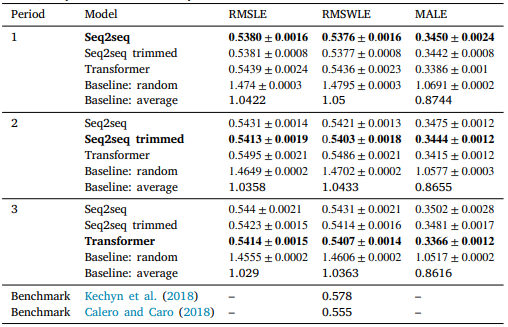
\includegraphics[width=0.7\textwidth]{2/figures/resul_ant2.png}
		\caption{Resultado antecedente}
		\textit{Fuente: Vallés-Pérez, I.(2022). Approaching sales forecasting using recurrent neural networks and transformers. Expert Systems with Applications, 201, 116993.}
		\label{fig9}
		
	\end{center}	
\end{figure}


%%%%%%%%%%%%%3

\subsection{Prediction Analysis Sales for Corporate Services Telecommunications Company using Gradient Boost Algorithm}

\subsubsection{Planteamiento del Problema y objetivo }
El documento se centra en la importancia de analizar y predecir las ventas en el ámbito empresarial, específicamente en una empresa de telecomunicaciones. Se destaca la relevancia de contar con estimaciones precisas para que la compañía pueda sobrevivir en un mercado competitivo y aumentar su crecimiento. Se menciona que el uso de técnicas de aprendizaje automático es fundamental para mejorar las predicciones futuras de ventas, ya que los sistemas de pronóstico tradicionales enfrentan dificultades al tratar con grandes volúmenes de datos y al intentar mejorar la precisión de las predicciones de ventas.
Se hace referencia a la necesidad de analizar la confiabilidad de las ventas de empresa a empresa (B2B) utilizando técnicas de aprendizaje automático. Se menciona que a lo largo de los años han surgido varios estudios que buscan predecir y pronosticar las ventas, y se destaca un sistema de análisis desarrollado utilizando métodos predictivos de aprendizaje automático. Se identificaron tres diferencias clave en los métodos alternativos para estimar las ventas de oportunidad, lo que llevó a una mejora significativa en la precisión de las predicciones.
Además, se menciona que el objetivo de la investigación es evaluar y analizar el uso de técnicas de aprendizaje automático para predecir las ventas, centrándose en las ventas B2B. Se describe el proceso de recopilación y preparación de datos, donde se utilizó información de ventas de tres años consecutivos (2016, 2017 y 2018) para predecir los ingresos B2B. Se destaca la importancia de seleccionar y procesar los datos relevantes para mejorar la precisión de las predicciones de ventas.


\subsubsection{Base de datos de los autores}
Utilizan un conjunto de datos de ventas anuales por producto para llevar a cabo el análisis de predicción de ventas en el contexto de ventas B2B para una empresa de telecomunicaciones. El conjunto de datos proporciona información detallada sobre las ventas de los productos MIDI y NO-MIDI durante los años 2016, 2017 y 2018, desglosadas por trimestre.
El conjunto de datos incluye información sobre las ventas en millones para cada trimestre de los años mencionados, tanto para los productos MIDI como para los productos NO-MIDI. Los datos incluían información detallada como categoría, región, tipo de artículo, ID de oportunidad, trimestre, nombre del producto, subcomponente del producto, producto de servicio (MIDI) e ingresos por ventas.


\subsubsection{Metodología empleada por los autores}

\begin{enumerate}
	\item Recopilación y Preparación de Datos: Se recopilaron datos de ventas de tres años consecutivos (2016, 2017 y 2018) para realizar el análisis de predicción de ingresos B2B. Se eliminaron datos no utilizables, redundantes e irrelevantes para obtener un conjunto de datos seleccionado que incluía trimestre, año, y elementos de servicio y cantidad.
	\item Preprocesamiento de Datos: Después de la preparación de datos, se llevó a cabo un estudio exploratorio para comprender la esencia de los resultados obtenidos. Se realizaron seis medidas esenciales de minería de datos, que incluyen conciencia de datos, planificación, simulación, evaluación e implementación.
	\item Se llevó a cabo la detección de valores atípicos como parte del proceso de optimización del modelo. La identificación de valores atípicos puede ser útil para mejorar el modelo o como punto de partida para futuras optimizaciones. Se hizo hincapié en la importancia de la calidad de los datos y se sugirió la eliminación de atributos de datos menos críticos.
	\item Eliminación de Atributos Menos Críticos: Se sugiere la eliminación de atributos de datos menos críticos que pueden no contribuir significativamente a la precisión de las predicciones. Esto ayuda a simplificar el modelo y mejorar su eficacia en la predicción de ventas B2B.
	\item Se presentan los resultados de la predicción en forma de tablas y gráficos que muestran las proyecciones de ventas para productos MIDI y NO-MIDI durante un período de cinco años. Estos resultados ayudan a visualizar las tendencias futuras y a tomar decisiones informadas sobre estrategias de ventas y presupuestos.
\end{enumerate}


%%%%%%%%%%%%%%%%4

\subsection{Predicting Future Sales of Retail Products using Machine Learning}

\subsubsection{Planteamiento del Problema y objetivo }
Sobre la predicción de ventas futuras de productos minoristas, se destaca la importancia de la precisión en la predicción de ventas para cualquier organización, ya sea una pequeña empresa o una empresa Fortune 500. Se menciona que esta precisión proporciona una estimación precisa del crecimiento de los ingresos de la empresa y puede utilizarse para planificar acciones de demanda y suministro a corto plazo. Además, sirve como guía para diseñar planes que se alineen con los objetivos organizacionales generales para la prudencia financiera.
Se menciona que el objetivo del proyecto es predecir las ventas totales de cada producto y tienda para el próximo mes utilizando datos pasados. Se destaca que se trabajó con un conjunto de datos desafiante de series temporales que consiste en datos de ventas diarias proporcionados por una de las mayores empresas de software de Rusia, la empresa 1C. Para realizar las predicciones del próximo mes, se implementaron el algoritmo eXtreme Gradient Boosting (XGBoost) y una arquitectura de red basada en Long Short Term Memory (LSTM) para realizar la tarea de aprendizaje.
Se menciona que la métrica utilizada para evaluar el rendimiento de los modelos y comparar los algoritmos implementados fue el error cuadrático medio de la raíz (RMSE). Además se destaca que XGBoost tuvo un mejor desempeño que LSTM en este conjunto de datos, lo que se atribuye a su relativa mayor dispersión.


\subsubsection{Base de datos de los autores}
El conjunto de datos es una combinación de datos de series temporales y datos estáticos. Los datos estáticos incluyen columnas como el nombre del artículo, la categoría del artículo, el ID de la tienda, etc., que no cambian con el tiempo, mientras que la cantidad de artículos y el precio del artículo varían con el tiempo. Se menciona que se siguió un proceso convencional de ingeniería de datos que incluyó limpieza de datos, análisis exploratorio de datos y creación de características.

\subsubsection{Metodología empleada por los autores}
La predicción de ventas futuras de productos minoristas fue un proceso fundamental para crear variables predictivas significativas a partir de los datos disponibles. A continuación, se presenta un resumen detallado de las acciones de ingeniería de características llevadas a cabo:

\begin{enumerate}
	\item Creación de un Conjunto de Datos Combinado: Se inició el proceso de ingeniería de características combinando todos los conjuntos de datos proporcionados, como los datos de tiendas, artículos y categorías de artículos, en un conjunto de datos maestro. Esta integración permitió tener una visión holística de la información disponible para el modelado predictivo.
	\item Generación de Características Basadas en Análisis Exploratorio: Se tomaron como base las observaciones del Análisis Exploratorio de Datos (EDA) para crear nuevas características relevantes. Por ejemplo, se crearon características relacionadas con el recuento de cada día de la semana en el bloque de fechas, el recuento de fines de semana y características estacionales basadas en el mes o la temporada.
	\item Incorporación de Información Temporal: Se extrajeron características temporales como retrasos temporales para capturar patrones de series temporales en los datos de ventas. Estas características incluyeron información sobre las ventas pasadas para cada producto y tienda, lo que permitió al modelo aprender de las tendencias históricas.
	\item Consideración de Variables Categóricas: Se realizaron transformaciones en variables categóricas, como la codificación one-hot encoding, para representarlas de manera adecuada en los modelos de aprendizaje automático. Esto incluyó la codificación de variables como la categoría del artículo o el ID de la tienda para que fueran interpretables por los algoritmos de predicción.\\
	
	\textbf{Modelos utilizados}
	
	\item XGBoost: Se seleccionó XGBoost como uno de los algoritmos iniciales debido a su amplia utilización en competiciones de ciencia de datos. XGBoost ofrece ventajas en términos de optimización del sistema a través de la paralelización y la optimización del hardware, así como la capacidad de manejar eficientemente diferentes patrones de esparsidad en los datos.
	\item ARIMA: Se incluyó el modelo ARIMA, ampliamente utilizado en series temporales, para comparar su rendimiento con otros modelos.
	\item LSTM: Se implementó una arquitectura basada en LSTM (Long Short-Term Memory) para modelar eficientemente características estáticas y dinámicas, inspirados en trabajos previos que demostraron la eficacia de combinar LSTM con redes neuronales totalmente conectadas.
	\item División de Datos: Se dividió el conjunto de datos en un conjunto de entrenamiento y un conjunto de validación, utilizando los primeros 32 meses para entrenar los modelos y el mes 33 para validar las predicciones.
	\item Ajuste de Hiperparámetros: Se realizó una búsqueda de hiperparámetros sobre un espacio de búsqueda utilizando muestreo aleatorio uniforme en el conjunto de validación para optimizar los modelos.
	\item Evaluación de Modelos: Se evaluaron los modelos en función de su capacidad para predecir las ventas futuras de productos y tiendas, considerando métricas de rendimiento como el error cuadrático medio (MSE) o el error absoluto medio (MAE).
	 
\end{enumerate}

\subsubsection{Resultados obtenidos}
Se encontró que XGBoost superó a los otros modelos, incluyendo ARIMA y LSTM, en la predicción de las ventas futuras de productos y tiendas. Se atribuyó el mejor rendimiento de XGBoost a la buena ingeniería de características y a la capacidad de ajustar una amplia gama de hiperparámetros durante la optimización.

\begin{table}[h!]
	\centering
	\begin{tabular}{lccc}
		\hline
		Modelo & RMSE de Entrenamiento & RMSE de Validación & RMSE de Prueba \\ \hline
		XGBoost & 0.76467 & 0.807264 & 0.87815 \\
		LSTM & 0.804657 & 0.898786 & 0.92417 \\
		ARIMA & 0.963426 & 0.9823224 & 1.09266 \\ \hline
	\end{tabular}
	\caption{Resultados antecedente}
	\textit{Fuente: Swami, D.(2020). Predicting future sales of retail products using machine learning. arXiv preprint arXiv:2008.07779.}

	\label{tabla:1}
\end{table}

\subsection{Time Series Forecasting and Modelling of Food Demand Supply Chain based on Regressors Analysis}

\subsubsection{Planteamiento del Problema y objetivo }
(\cite{Pandasandeep2023}) El sector de entrega de alimentos enfrenta grandes desafíos en la gestión de inventarios, ya que la demanda de comidas puede ser altamente variable debido a factores como cambios estacionales, promociones y fluctuaciones en las preferencias de los clientes. Este comportamiento errático de la demanda complica la planificación de la producción y puede llevar a la empresa a sufrir pérdidas económicas. La sobreproducción de alimentos puede ocasionar desperdicio y costos innecesarios, mientras que la subproducción puede resultar en una escasez de productos, afectando la satisfacción del cliente y la lealtad hacia la marca.
El objetivo principal de esta investigación es desarrollar un modelo de pronóstico de demanda que permita predecir con precisión el número de pedidos de comidas para las próximas 10 semanas. Con este modelo, la empresa puede optimizar la gestión de inventarios, minimizando el desperdicio de alimentos y los costos operativos, al mismo tiempo que mejora la disponibilidad de productos y la satisfacción del cliente. Al anticipar la demanda, la empresa podrá tomar decisiones más informadas sobre compras y producción, aumentando su eficiencia operativa y rentabilidad.
Para llevar a cabo este estudio, se utilizó un conjunto de datos que abarca 145 semanas de pedidos semanales de 50 comidas diferentes, lo que proporciona un total de aproximadamente 450,000 entradas. Cada entrada incluye 15 características, entre ellas, el número de ventas, los precios, los descuentos aplicados, el centro de distribución, y otros atributos que influyen en la demanda. La importancia de este problema radica en que una predicción inexacta puede desencadenar una serie de problemas logísticos y financieros, afectando el rendimiento global de la empresa de entrega de alimentos.


\subsubsection{Base de datos de los autores}
El conjunto de datos, denominado ``Food Demand Forecasting'', fue proporcionado por Genpact, una firma de servicios profesionales especializada en el análisis de datos empresariales. Este conjunto incluye registros históricos detallados de los pedidos realizados semanalmente para diferentes tipos de comidas. Los datos se distribuyen en tres archivos, los cuales contienen columnas como el ID del pedido, el número de semana, el ID de la comida, el ID del centro de cumplimiento, y el precio final.
Los datos originales estaban en un formato heterogéneo y requirieron una preparación significativa para su uso en los modelos predictivos. Se aplicaron técnicas de limpieza y normalización para eliminar registros incompletos y valores atípicos que pudieran afectar la precisión del modelo. Además, se añadieron características adicionales, como medias móviles para capturar tendencias a corto plazo y características de rezago para incluir información histórica en el modelo. La construcción de estas nuevas características permitió enriquecer la información y mejorar la capacidad del modelo para detectar patrones en la demanda.


\subsubsection{Metodología empleada por los autores}

\begin{enumerate}
\item \textbf{Modelos Utilizados:} La metodología incluyó la utilización de varios modelos de machine learning y deep learning, con el objetivo de comparar su desempeño en la predicción de la demanda de comidas. Los modelos probados incluyeron Random Forest Regressor, Gradient Boosting Regressor, LightGBM, XGBoost, CatBoost Regressor, LSTM (Long Short-Term Memory) y BiLSTM (Bidirectional Long Short-Term Memory). La selección de estos modelos se basó en su capacidad para capturar relaciones no lineales y temporales en los datos.
\item \textbf{Etapas del Proceso:} El proceso se dividió en varias etapas. Inicialmente, se realizó la preparación de los datos, que incluyó la limpieza, normalización y creación de nuevas características. Posteriormente, se llevó a cabo el entrenamiento de los modelos utilizando un conjunto de datos que cubría 113 semanas. Para validar la precisión del modelo y ajustar los hiperparámetros, se utilizó un subconjunto de 10 semanas. Finalmente, se emplearon las últimas 10 semanas de datos para probar y evaluar el desempeño de los modelos.
\item \textbf{Herramientas y Tecnologías:} Para la implementación de los modelos, se utilizaron lenguajes de programación como Python y herramientas específicas de machine learning y deep learning. Entre los frameworks empleados destacan TensorFlow, Keras y scikit-learn, los cuales permitieron construir y entrenar redes neuronales complejas. Además, se utilizaron pandas y NumPy para el manejo y preprocesamiento de los datos, y Matplotlib y Seaborn para la visualización de resultados.
\item \textbf{Procedimientos Implementados:} Se inició definiendo las estructuras de las redes neuronales, seleccionando el número de capas y neuronas adecuadas para captar las relaciones complejas entre las variables. Para los modelos de LSTM y BiLSTM, se prestó especial atención a la configuración de los hiperparámetros, como el número de épocas de entrenamiento, la tasa de aprendizaje y el tamaño de las secuencias de entrada. A lo largo del proceso, se llevaron a cabo múltiples iteraciones de entrenamiento para optimizar los modelos y mejorar la precisión en las predicciones.
\item \textbf{Optimización de Modelos:} Además de entrenar los modelos, se implementaron técnicas de optimización, como la búsqueda de hiperparámetros (Grid Search y Random Search) para encontrar la configuración más eficaz. También se aplicaron técnicas de regularización y ``early stopping''
 para prevenir el sobreajuste del modelo durante el entrenamiento.
\item \textbf{Evaluación de Resultados:} Se evaluó el desempeño de los modelos utilizando métricas como RMSLE (Root Mean Squared Logarithmic Error), RMSE (Root Mean Squared Error), MAPE (Mean Absolute Percentage Error) y MAE (Mean Absolute Error). Estas métricas proporcionaron una visión detallada de la precisión y robustez de cada modelo al predecir la demanda.
\end{enumerate}

\subsubsection{Resultados obtenidos}
Los resultados mostraron que los modelos de deep learning, en particular el modelo LSTM, superaron a los demás en términos de precisión al predecir la demanda de comidas. Las métricas de evaluación para el modelo LSTM incluyeron un RMSLE de 0.28, un RMSE de 18.83, un MAPE de 6.56\% y un MAE de 14.18. Estas cifras indicaron un alto nivel de precisión en las predicciones, lo que lo convierte en una herramienta eficaz para la planificación de inventarios.
Durante la evaluación, se realizó una comparación detallada entre los valores reales y los pronosticados por el modelo. Los resultados mostraron una fuerte correlación entre las predicciones y los valores reales, validando así la efectividad del modelo LSTM para capturar las tendencias y patrones de la demanda. Este análisis demostró que la implementación del modelo propuesto puede ayudar a las empresas de entrega de alimentos a gestionar sus inventarios de manera más eficiente, reduciendo los costos asociados al desperdicio de alimentos y mejorando la satisfacción del cliente.

\begin{table}[h!]
	\centering
	\begin{tabular}{lcccc}
		\hline
		Models/Metrics & RMSLE & RMSE & MAPE & MAE \\ \hline
		 Random Forest & 0.35 &  228.92 & 10.822 & 115.90 \\
		 Gradient Boost & 0.31 & 226.46 & 10.03 & 123.48 \\
		 Light Boost & 0.31 & 194.68 & 10.08 & 104.49 \\
		 XGB & 0.30 & 205.31 & 9.97 & 106.17\\
		 CatBoost & 0.29 & 186.68 & 9.76 & 99.40 \\
		 LSTM & 0.28 & 18.83 & 6.56 & 14.18 \\
		 Bi-LSTM & 0.37 & 31.88 & 12.8 & 28.33 \\ \hline
		
	\end{tabular}
	\caption{Resultados antecedente}
	\textit{Fuente: Kumar, P. (2023). Time Series Forecasting and Modeling of Food Demand Supply Chain Based on Regressors Analysis. IEEE Access}
	
	\label{tabla:15}
\end{table}

\subsection{Advancing Retail Predictions: Integrating Diverse Machine Learning Models for Accurate Walmart Sales Forecasting}

\subsubsection{Planteamiento del Problema y objetivo}
(\cite{nebacyril2024}) En el sector minorista, la previsión precisa de las ventas es un desafío constante. Los errores en las predicciones pueden tener un impacto significativo en la gestión de inventarios, llevando a problemas como el exceso de productos o su escasez. Estos problemas, a su vez, afectan negativamente la satisfacción del cliente, las operaciones y la rentabilidad de la empresa. Walmart, como líder en el sector retail, necesita un sistema robusto que le permita anticipar la demanda para optimizar sus estrategias de abastecimiento, compras y promociones.

El objetivo de esta investigación es desarrollar un sistema de pronóstico de ventas que utilice modelos de machine learning para mejorar la precisión de las predicciones de ventas en Walmart. Un sistema más preciso permitirá una mejor gestión del inventario, reducir costos asociados con el exceso o falta de stock, y optimizar la toma de decisiones estratégicas, especialmente durante períodos críticos como temporadas de vacaciones o cambios económicos.
Para abordar este problema, se utilizaron datos históricos de ventas de Walmart que abarcan desde febrero de 2010 hasta octubre de 2012. Los datos incluyen una amplia variedad de variables como banderas de vacaciones, temperatura, precios de combustible, el Índice de Precios al Consumidor (CPI), tasas de desempleo y las ventas semanales. La inclusión de estas variables externas permitió al modelo captar patrones y relaciones más complejas en la variabilidad de la demanda.

\subsubsection{Base de datos de los autores}
El conjunto de datos fue obtenido de Kaggle, una plataforma que proporciona datasets para análisis y modelos predictivos. El dataset específico contiene información sobre las ventas de Walmart en diferentes tiendas y departamentos a lo largo de un período de casi tres años. Los datos están organizados en un formato tabular, con columnas que incluyen fechas, ventas semanales, identificadores de tienda y departamento, y variables externas como el clima y condiciones económicas.

Para asegurar la calidad de la información, se realizó un exhaustivo proceso de preparación de los datos. Esto incluyó la normalización de las variables, la eliminación de valores atípicos que pudieran distorsionar el modelo, y el manejo de valores faltantes. Durante esta etapa, se incorporaron características adicionales relevantes, como la extracción de información temporal (día de la semana, mes, año) y la identificación de períodos de alta demanda, como días festivos, para ayudar al modelo a captar mejor las tendencias y patrones estacionales.

\subsubsection{Metodología empleada por los autores}
\begin{enumerate}
	\item \textbf{Modelos de Machine Learning Utilizados:} Se probaron varios modelos de machine learning para identificar cuál proporcionaba las predicciones más precisas. Entre los modelos evaluados se incluyeron la Regresión Lineal, Random Forest, Gradient Boosting Machines (GBM), eXtreme Gradient Boosting (XGBoost) y Light Gradient Boosting Machine (LightGBM). Estos modelos fueron seleccionados por su capacidad para manejar datos complejos y relaciones no lineales entre las variables.
	\item \textbf{Etapas del Proceso:}
	\begin{itemize}
		\item \textbf{Preparación de Datos:} La primera etapa del proceso consistió en la recolección, limpieza y normalización de los datos. Los datos se dividieron en conjuntos de entrenamiento y validación para garantizar que el modelo fuera capaz de generalizar a nuevas situaciones. También se realizó una transformación de variables, como la creación de características temporales y la codificación de variables categóricas.
		\item \textbf{Entrenamiento del Modelo:} Se entrenaron los modelos seleccionados utilizando el conjunto de datos de entrenamiento. Durante esta etapa, se realizaron ajustes a los hiperparámetros de los modelos para optimizar su rendimiento, empleando técnicas como la búsqueda en cuadrícula (Grid Search) y la validación cruzada.
		\item \textbf{Validación:} Una vez entrenados los modelos, se validó su rendimiento utilizando el conjunto de datos de validación. Las métricas de evaluación incluyeron el Error Absoluto Medio (MAE), la Raíz del Error Cuadrático Medio (RMSE) y el Coeficiente de Determinación (R-squared). Estas métricas proporcionaron una visión completa de la precisión y robustez de cada modelo al predecir las ventas.
	\end{itemize}
	\item \textbf{Herramientas y Tecnologías Utilizadas:} Para implementar y entrenar los modelos, se utilizaron lenguajes de programación como Python junto con bibliotecas y frameworks especializados en machine learning, tales como scikit-learn y XGBoost. El uso de estas herramientas permitió construir modelos complejos y eficientes en términos computacionales, además de facilitar el análisis y visualización de resultados.
	\item \textbf{Procedimientos Implementados:} Durante el proceso de desarrollo del modelo, se definieron las estructuras de los algoritmos y se realizaron ajustes de hiperparámetros para optimizar su desempeño. Se implementaron técnicas de regularización y selección de características para mejorar la capacidad predictiva de los modelos y reducir el riesgo de sobreajuste. Además, se realizaron múltiples iteraciones de entrenamiento y prueba para garantizar que los modelos fueran capaces de adaptarse a las diferentes condiciones representadas en los datos históricos.
\end{enumerate}

\subsubsection{Resultados obtenidos}
Los resultados del estudio mostraron que los modelos avanzados, especialmente XGBoost, proporcionaron un nivel de precisión superior en comparación con otros modelos más simples. El modelo XGBoost obtuvo un Error Absoluto Medio (MAE) de 1226.471, un RMSE de 1700.981, y un R-squared de 0.9999900, lo que indica una precisión casi perfecta en las predicciones. Este desempeño demuestra la capacidad del modelo para adaptarse a las complejas relaciones entre las variables y capturar las fluctuaciones en la demanda de ventas de Walmart.
En contraste, los modelos más simples como la Regresión Lineal mostraron un rendimiento significativamente menor, con un MAE de 35632.510 y un RMSE de 80153.858. Esta diferencia destaca la importancia de utilizar algoritmos avanzados para abordar problemas de predicción complejos en el entorno minorista.
Adicionalmente, se realizó un análisis de sesgo y equidad para evaluar el rendimiento de los modelos en diferentes segmentos temporales, como períodos de vacaciones y no vacaciones. Los resultados indicaron que los modelos avanzados, en particular XGBoost, lograron minimizar los errores de predicción y mantener un rendimiento equilibrado incluso en los períodos de alta variabilidad de la demanda.

\begin{table}[h!]
	\centering
	\begin{tabular}{lcccc}
		\hline
		Model & MAE & RMSE & R Squared  \\ \hline
		Linear Regression & 35632.510 &  80153.858 & 0.9760562  \\
		Multiple Regression & 35632.510 & 80153.858 & 0.9760562 \\
		GLM & 35632.510 & 80153.858 & 0.9760562 \\
		Decision Tree & 77388.082 & 93721.066 & 0.9696449 \\
		Ramdom Forest & 12238.782 & 19814.965 & 0.9986431 \\
		GBM & 10839.822 & 1700.981 & 0.9993119 \\
		XGBoost & 1226.471 & 1700.981 & 0.9999900 \\
		LGB & 1692.640 & 2297.930 &  0.9999818\\ \hline
		
	\end{tabular}
	\caption{Resultados de modelos predictivos}
	\textit{Fuente: Cyril, N. (2024). Advancing Retail Predictions: Integrating Diverse Machine Learning Models for Accurate Walmart Sales Forecasting. Asian Journal of Probability and Statistics}
	
	\label{tabla:15}
\end{table}


\subsection{Demand Forecasting for Online Market Stock: Case study Cleanroom Apparel}

\subsubsection{Planteamiento del Problema y objetivo}
El problema del estudio se centra en la necesidad de crear un marco de pronóstico apropiado para la planificación de la demanda de producción de las pequeñas y medianas empresas (PYMES). Estas empresas a menudo enfrentan desafíos debido a la variabilidad en las ventas de productos y la falta de técnicas de pronóstico efectivas, lo que puede resultar en exceso de inventario o escasez de productos. Esto se debe a que las decisiones de producción a menudo se basan en la experiencia de los empleados, lo que no siempre responde a la demanda del cliente.

El objetivo del estudio es analizar y desarrollar un marco de pronóstico que permita prever la demanda de productos, particularmente para los cinco productos más vendidos por la empresa. Para lograr esto, se utilizan una variedad de técnicas de predicción, como el promedio móvil, el suavizado exponencial y el análisis de regresión, para determinar el método más efectivo para reducir el error de predicción y optimizar la cantidad económica de pedido ademas de los costos totales asociados con la producción y el inventario.

\subsubsection{Base de datos de los autores}
El estudio utilizó una base de datos de ventas de productos de una empresa de 2015 a 2017.\\
Estos son los elementos clave de esta base de datos:

\begin{enumerate}
	\item {Productos Analizados: Se seleccionaron los cinco productos más vendidos, que se denominaron A, B, C, E y L.}
	\item{Recopilación de información: La base de datos contiene datos sobre:}
	\begin{itemize}
		\item{La cantidad de unidades vendidas de cada producto durante el período mencionado se conoce como demanda.}
		\item{El precio de cada producto es el precio unitario.}
		\item{El valor total de ventas de cada producto se puede calcular multiplicando la demanda por el precio.}	
	\end{itemize}
	
	\item{Formato de Presentación: Una tabla con columnas para el nombre del producto, la demanda total, el precio por unidad y el valor total de ventas contiene los datos. Por ejemplo, la tabla muestra que el Producto A tuvo una demanda de 14,110 unidades al precio de 530 Baht, lo que resultó en un valor total de ventas de 7,478,300 Baht.}
	\item{Objetivo de los datos: Estos datos se utilizan para aplicar una variedad de técnicas de pronóstico y determinar cuál es la más efectiva para prever la demanda futura. También se utilizan para determinar la cantidad económica de pedido (EOQ) y los costos totales relacionados con la gestión del inventario.}
\end{enumerate}


\subsubsection{Metodología empleada por los autores}

\begin{enumerate}
	\item Recolección de Datos
	\begin{itemize}
		\item Origen de los Datos: Se obtuvieron datos de ventas de productos de una empresa durante los años 2015 a 2017.
		\item Selección de Productos: Se identificaron los cinco productos más vendidos, denominados Producto A, B, C, E y L.
	\end{itemize}
	
	\item Análisis de la Información
	\begin{itemize}
		\item Características de los Datos: Se examinaron aspectos clave de los datos de ventas, tales como la demanda total, el precio unitario y el valor total de ventas para cada producto.
		\item Organización de los Datos: Los datos fueron presentados en tablas que detallan la demanda, el precio y el valor total de cada producto.
	\end{itemize}
	
	\item Selección de Técnicas de Pronóstico
	\begin{itemize}
		\item Métodos Comparados: Se seleccionaron cuatro métodos de pronóstico para evaluar su precisión:
		\begin{enumerate}
			\item Promedio Móvil
			\item Suavizado Exponencial Simple
			\item Suavizado Exponencial Doble
			\item Análisis de Regresión
		\end{enumerate}
	\end{itemize}
	
	\item Aplicación de Técnicas de Pronóstico
	\begin{itemize}
		\item Implementación: Se aplicaron los métodos seleccionados a los datos de ventas de los cinco productos para estimar la demanda futura.
		\item Cálculo de Errores: Se midió la precisión de cada pronóstico utilizando el Error Absoluto Porcentual Medio (MAPE).
	\end{itemize}
	
	\item Identificación del Método Más Eficiente
	\begin{itemize}
		\item Comparación de Resultados: Se contrastaron los valores de MAPE para determinar cuál método proporcionó el pronóstico más exacto para cada producto.
		\item Selección del Método: Se eligió el método con el menor MAPE como el más adecuado para cada producto.
	\end{itemize}
	
	\item Cálculo de la Cantidad Económica de Pedido
	\begin{itemize}
		\item Cálculo de EOQ: Después de seleccionar el método de pronóstico más preciso, se determinó la cantidad económica de pedido para cada producto, optimizando la gestión de inventario.
		\item Evaluación de Costos: Se calcularon los costos totales asociados a la administración del inventario, utilizando los pronósticos y la EOQ obtenidos.
	\end{itemize}
	
	\item Interpretación de Resultados
	\begin{itemize}
		\item Visualización: Los resultados fueron representados mediante gráficos que muestran la demanda de cada producto a lo largo del tiempo.
		\item Conclusiones: Se discutieron las repercusiones de los resultados en la gestión de inventario y la satisfacción del cliente, así como recomendaciones para investigaciones futuras.
	\end{itemize}
\end{enumerate}


\subsubsection{Resultados obtenidos}
\textbf{Producto A}
\begin{itemize}
	\item Método de Pronóstico Utilizado: Análisis de Regresión
	\item MAPE: 22.03
	\item Cantidad Económica de Pedido (EOQ): 172 unidades
	\item Costo Total: 27,345.51 Baht
\end{itemize}

\textbf{Producto B}
\begin{itemize}
	\item Método de Pronóstico Utilizado: Suavizado Exponencial Simple
	\item Valor de $\alpha$: 0.056
	\item MAPE: 72.20
	\item Cantidad Económica de Pedido (EOQ): 150 unidades
	\item Costo Total: 23,280.66 Baht
\end{itemize}

\textbf{Producto C}
\begin{itemize}
	\item Método de Pronóstico Utilizado: Análisis de Regresión
	\item MAPE: 28.10
	\item Cantidad Económica de Pedido (EOQ): 193 unidades
	\item Costo Total: 24,953.52 Baht
\end{itemize}

\textbf{Producto E}
\begin{itemize}
	\item Método de Pronóstico Utilizado: Promedio Móvil ($n=3$)
	\item MAPE: 31.50
	\item Cantidad Económica de Pedido (EOQ): 336 unidades
	\item Costo Total: 14,109.57 Baht
\end{itemize}

\textbf{Producto L}
\begin{itemize}
	\item Método de Pronóstico Utilizado: Análisis de Regresión
	\item MAPE: 47.00
	\item Cantidad Económica de Pedido (EOQ): 1844 unidades
	\item Costo Total: 6,639.97 Baht
\end{itemize}

\textbf{Análisis de Resultados}
\begin{itemize}
	\item \textbf{Efectividad de los Métodos}: El análisis de regresión demostró ser el método más efectivo para los Productos A y C, mientras que el suavizado exponencial simple fue el más adecuado para el Producto B. El promedio móvil fue el mejor para el Producto E.
	\item \textbf{Variación en EOQ}: Las cantidades económicas de pedido (EOQ) varían significativamente entre los productos, con el Producto L requiriendo la mayor cantidad de 1844 unidades, lo que indica una alta demanda o un costo de mantenimiento bajo en comparación con otros productos.
	\item \textbf{Costos Totales}: Los costos totales asociados a la gestión del inventario también varían, reflejando las diferencias en la demanda y la cantidad de pedido óptima.
\end{itemize}



%%%%%%%%%%%%%%%%%4
%\subsection{Inteligencia Empresarial y Análisis de Datos: De Big Data a Gran Impacto}
%
%\textbf{Resumen:} El artículo examina el papel crucial de la inteligencia empresarial y el análisis de datos, especialmente en el contexto del análisis de big data, en la mejora de la rentabilidad y la toma de decisiones en las organizaciones. Se centra específicamente en la aplicación de estas herramientas para predecir la demanda de productos perecibles, lo que puede resultar en mejoras significativas en la eficiencia operativa y la rentabilidad. Objetivo: Analizar cómo las empresas pueden aprovechar la inteligencia empresarial y el análisis de big data para mejorar la predicción de la demanda de productos perecibles y, en última instancia, aumentar su rentabilidad. \textbf{Metodología:} Se empleó una metodología que combina una revisión teórica con el análisis de casos de empresas que han implementado soluciones de big data para la predicción de la demanda. Se examinan estudios de casos y ejemplos concretos para ilustrar cómo estas tecnologías pueden impactar en la rentabilidad y la toma de decisiones empresariales. \textbf{Resultados:} Se resalta la importancia estratégica de la inteligencia empresarial y el análisis de datos en la mejora de la rentabilidad y la toma de decisiones en las organizaciones. Conclusiones: El uso efectivo del big data puede conducir a mejoras significativas en la rentabilidad, especialmente a través de la predicción precisa de la demanda de productos perecibles. Se recomienda a las empresas invertir en tecnologías y capacidades de análisis de datos para aprovechar al máximo este potencial.
%
%\subsection{Pronóstico de la Demanda de Productos Perecibles: Una Revisión de la Literatura}
%
%\textbf{Resumen:} Este artículo proporciona una revisión exhaustiva de la literatura sobre el pronóstico de la demanda de productos perecibles. Se enfoca en la importancia del pronóstico preciso de la demanda para una gestión efectiva de productos perecibles, y cómo diferentes enfoques pueden influir en la precisión de los pronósticos. \textbf{Objetivo:} Revisar y analizar críticamente la literatura existente sobre el pronóstico de la demanda de productos perecibles, identificando las principales técnicas y enfoques utilizados en este campo y su impacto en la gestión de inventarios y la rentabilidad. \textbf{Metodología:} Se utilizó una metodología de revisión sistemática de la literatura para examinar una amplia gama de investigaciones y estudios sobre pronóstico de la demanda. Se analizaron diferentes enfoques, incluyendo métodos estadísticos tradicionales y modelos basados en big data, para evaluar su efectividad en la predicción de la demanda de productos perecibles. Resultados: Se identificaron y discutieron las principales técnicas utilizadas en el pronóstico de la demanda de productos perecibles, así como sus ventajas y desventajas. \textbf{Conclusión:} El pronóstico preciso de la demanda es esencial para minimizar el desperdicio y optimizar la gestión de inventario en productos perecibles. Se sugiere que las empresas deben considerar una combinación de enfoques para mejorar la precisión de los pronósticos de demanda. 
%
%
%\subsection{Análisis y Predicción de Tendencias Criminales mediante Big Data Analytics y Mining}
%\textbf{Resumen:} El artículo aborda la predicción de tendencias criminales a través de un análisis exploratorio de datos en ciudades como San Francisco, Chicago y Filadelfia, empleando técnicas avanzadas de Big Data y Deep Learning. Se utilizan métodos como Deep Learning, Series Temporales y Big Data, y se implementan modelos como Prophet y Keras stateful LSTM, además de visualizar la información en un mapa geográfico. Objetivo: Analizar datos públicos de delincuencia en San Francisco, Chicago y Filadelfia, con registros que abarcan diferentes periodos de tiempo en cada ciudad. \textbf{Metodología:} El proceso comienza con el preprocesamiento de datos, que incluye la división de la variable de fecha y el manejo de datos faltantes mediante el uso de la media. Se emplean tres métodos para elaborar los modelos: el Modelo Prophet, Redes Neuronales y LSTM (Long Short-Term Memory), cada uno con características específicas. \textbf{Resultados:} El rendimiento de los modelos se evalúa utilizando métricas como el Error Cuadrático Medio de la Raíz (RMSE) y la correlación de Spearman, variando parámetros y tamaños de muestra para todos los modelos. \textbf{Conclusiones:} Se determina que el periodo óptimo de previsión es de 3 años, con valores de RMSE y correlación de Spearman óptimos.
%
%\subsection{Aplicaciones Predictivas de Big Data Analytics en la Gestión de la Cadena de Suministro}
%\textbf{Objetivo:} El artículo se centra en la creciente atención que está recibiendo la analítica de datos grandes (BDA) en la gestión de la cadena de suministro (SCM), dada su amplia gama de aplicaciones, incluyendo el análisis del comportamiento del cliente, el análisis de tendencias y la predicción de la demanda. La investigación se enfoca en las aplicaciones predictivas de BDA en la previsión de la demanda en la cadena de suministro, con el objetivo de proponer una clasificación de estas aplicaciones, identificar brechas y proporcionar ideas para futuras investigaciones. \textbf{Metodología:} Se lleva a cabo una encuesta para investigar las aplicaciones predictivas de BDA en la previsión de la demanda en la cadena de suministro.  \textbf{Resultados:} Se destaca la falta de aplicaciones de BDA para la previsión de la demanda en el caso de cadenas de suministro de bucle cerrado (CLSC). Se identifican brechas en la literatura y se proponen vías para futuras investigaciones.